\section{Product Perspective}
In subsection \textit{2.1.1} are listed the most relevant scenarios which are a narrative description of what users do and experience as they try to make use of the application.\\
They provide a general depiction of how major components of the system and users interact.\\
Moreover, in subsections \textit{2.1.2} and \textit{2.1.3} the domain of the system is defined through different models using UML.

\subsection{Scenarios}

\begin{enumerate}

\item Scenario: \textbf{Sunil discovers DREAM}\\\\
Sunil is a farmer from Telangana. Unfortunately, due to the adverse and unpredictable effects of climate change, his production of black carrots is gradually decreasing. Sunil learns from a colleague of his that there is an application called DREAM that could help him. Sunil registers and logs in, hoping to profit from it and improve his production.\\

\item Scenario: \textbf{Rajesh looking for advice}\\\\
Rajesh is a landowner from Adilabad district in Telangana, he owns several agricultural properties in the city. After his recent business trip to Russia, where he attended the beet fair, he is convinced to plant beets on his land too. As this is a little-known plant in the area, he doesn't know who to ask for advice. Rajesh's son Ram, also in the agricultural sector for several years, advises his father to use DREAM since Rajesh already had an account registered with the application.
Rajesh consults on the application the discussions already opened by other Telangana farmers to see if any of them had ever sought advice on beet cultivation. Unfortunately he cannot find any, so thanks to the suggestion of his son Ram he decides to open a thread on the dedicated forum, so that he can ask for advice about the plant from other farmers throughout Telangana.\\

\item Scenario: \textbf{Anita and her strategic plan}\\\\
Anita is the administrator of her mandal Sarangapur, in Jagtial district, as an inspector of production and development of the primary sector. Sarangapur is characterized by great periods of drought, so water is a particularly precious resource for citizens.
Recent analyzes have shown that over 90\% of the water is used by farmers.
Anita discovers DREAM and she wants to monitor the water consumption within each mandal in Telangana over the current year. Her goal is to identify the one that consumes the least water to study its strategies, so she enters the parameters of interest (quantity of water and Telangana mandals) on the application.
At this point the app returns the mandals and the corresponding consumed water in this last year and Anita is pleased to discover that the primacy is Pegadapalli, a mandal from her own district.\\

\item Scenario: \textbf{Manoj, the Indian tycoon}\\\\
Manoj is an Indian tycoon who would like to invest his capital in the agricultural sector. He accesses the DREAM application as policy maker and checks the map showing the performance score of each mandal. Manoj identifies the best performing ones and decides to invest in Geesugonda mandal which is located in Warangal district.\\

\item Scenario: \textbf{Mahima is thrilled with joy for DREAM}\\\\
Mahima is the Additional Director of Agriculture who assist the state Head quarter Commissioner\&Director of Agriculture in Telangana. She belongs to the Department of Agriculture, which provides agricultural services to farmers and aims to transfer the latest technical knowledge to the farming community. She was one of those who pushed for the creation of DREAM.
Mahima is thrilled with joy for its market launch and she is looking forward to use the application, therefore she gets her personal ID code to be able to registers with the role of policy maker and logs into DREAM.\\

\item Scenario: \textbf{A new job for Shanti}\\\\
Shanti is a young agronomist who operated in Palakeedu, a mandal in Suryapet district. She sees the announcement published on the Telangana government website in which it is reported that the DREAM application has been launched on the market and that for each mandal is required an agronomist. She is unemployed and interested in filling this role. Therefore, she sends her CV, gets hired and receives her personal ID code which allows her to register into DREAM. Eventually, she inserts Palakeedu as mandal of her competence.\\

\item Scenario: \textbf{Champak tries natural farming}\\\\
Champak is a farmer who has planted wheat. The last crop was poor because he didn't have enough money to buy suitable pesticides. He still can't afford them, however he cannot suspend his agricultural activity since his family depends on it as the principal means of livelihood. For this reason Champak creates a help request to both the agronomist and well performing farmers. The first to answer is Jayapal, a well performing farmer from his same mandal. Jayapal suggests him to plant potatoes instead of wheat because they are more resistant. However, Champak has already planted wheat therefore changing crops is out of the question. Champak waits for other answers until Rajat, the agronomist, replies suggesting him to cover the seeds with microorganisms obtained from particular formulations of cow dung. Champak is willing to follow the advice and is satisfied with the answer. He marks the help request as solved. 
\\

\item Scenario: \textbf{The busy life of Aruna}\\\\
Aruna is the DREAM agronomist responsible for Jaipur mandal in Mancherial district. It is early morning and the working day is about to begin. Aruna consults the daily plan to check which are the scheduled visits for the day. An appointment with the farmer Gangesh is scheduled for the afternoon. At that moment she receives a phone call from him, who informs her that his wife is not well, he has to take her to the doctor and for this he has to cancel the scheduled visit. Aruna wishes him the best and updates the daily plan, cancelling the appointment. Further on, she completes all the appointments scheduled in the morning and she drives her car to reach Jaya, a farmer. Unfortounately, Aruna has a small accident with her car, she is unharmed but she will miss the appointment. She informs Jaya and calls a mechanic. She finally returns home in the evening and confirms the daily plan, also specifying the deviation corresponding to the missed visit due to the accident. She also has to reschedule in the first two free slots in her agenda the appointments with Jaya and Gangesh. To do so, she updates the daily plan of the next day. 
\\
\item Scenario: \textbf{Durvish, the inspector}\\\\
Durvish is the administrative head of Doma mandal, in Vikarabad district. The DREAM application was launched on the market the year before and now he wants to understand whether the steering initiatives carried out by agronomists with the help of good farmers have produced significant results. Therefore, Durvish accesses DREAM with his account and he enters the parameters of interest on the application to select only farmers of his mandal with at least an Help Request solved.
At this point the app returns the selected farmers. Durvish wants to visualize their general trend of the performance score as indicator of the efficiency of the application. He selects score as attribute and mean as operation, in return a time chart is shown. He pleasantly discovers that, except for an initial fluctuating trend, the general performance score of farmers with at least a solved Help Request of his mandal is constantly growing, a sign of effective usefulness of DREAM.
\\

\item Scenario: \textbf{Deepa fights soil salinity}\\\\
Deepa is a farmer of Telangana who is already using the application DREAM. The cotton she planted is now ready for harvest. The amount of cotton obtained from her hectare of land results in 3 bales, which correspond approximately to 107 kg each. Deepa accesses the app, selects the date corresponding to the current day and inserts in the system type and quantity of product harvested. Two days later, while approaching to plant cotton seeds again, she has a problem regarding the salinity of the soil which is particularly high and would not allow cotton to grow. For this reason, Deepa stores this information in the system selecting the current day, also adding that it was necessary to buy a biostimulant whose formulation neutralizes excess salts within the soil.
\\

\item Scenario: \textbf{Haresh's first encounter with coffee}\\\\
Haresh is a farmer of Telangana who is already using the application DREAM. It is October and within a few days he will have to harvest the sorghum he has planted. To better organize the work of the next few days, Haresh accesses the application and checks the weather forecasts. After the harvest he will also have to decide what to plant, which is why he also checks the soil moisture. Furthermore, due to the drought expected for November, the app suggests Haresh to plant coffee, a product that does not require a particularly humid soil. Haresh thinks that it could be a good idea, however he has never cultivated coffee so it could be necessary to confront with the agronomist about some technical details. Haresh doesn't remember when his next visit with the agronomist will occur, therefore he accesses the visits page on the application and pleasantly reads that one is scheduled for November 5th.
\\

\item Scenario: \textbf{Lohit helps the most needy}\\\\
Lohit is the DREAM agronomist responsible for Raipole mandal in Siddipet district. The performance score in his mandal for a good percentage of farmers has been around a value that has not been particularly high for more than six months. For this reason Lohit wants to visualize data regarding best performing farmers to formulate strategies to be applied to the most needy. He accesses DREAM and visualizes farmers whose performance score is between the highest. Analyzing the corresponding data he finds out that they cultivate all the same type of product: rice, which is cultivable under widely varying conditions but prefers hot and humid climate. Therefore, before advising other farmers to plant rice, Lohit consults weather forecasts and humidity of soil trend, discovering that with a very high probability there will be the perfect conditions in the next weeks.
\\

\end{enumerate}

\newpage
\subsection{Class Diagram}
In this section is reported the Class Diagram of the System, whose main concepts are presented from a high-level point of view. 
\begin{figure}[H]
  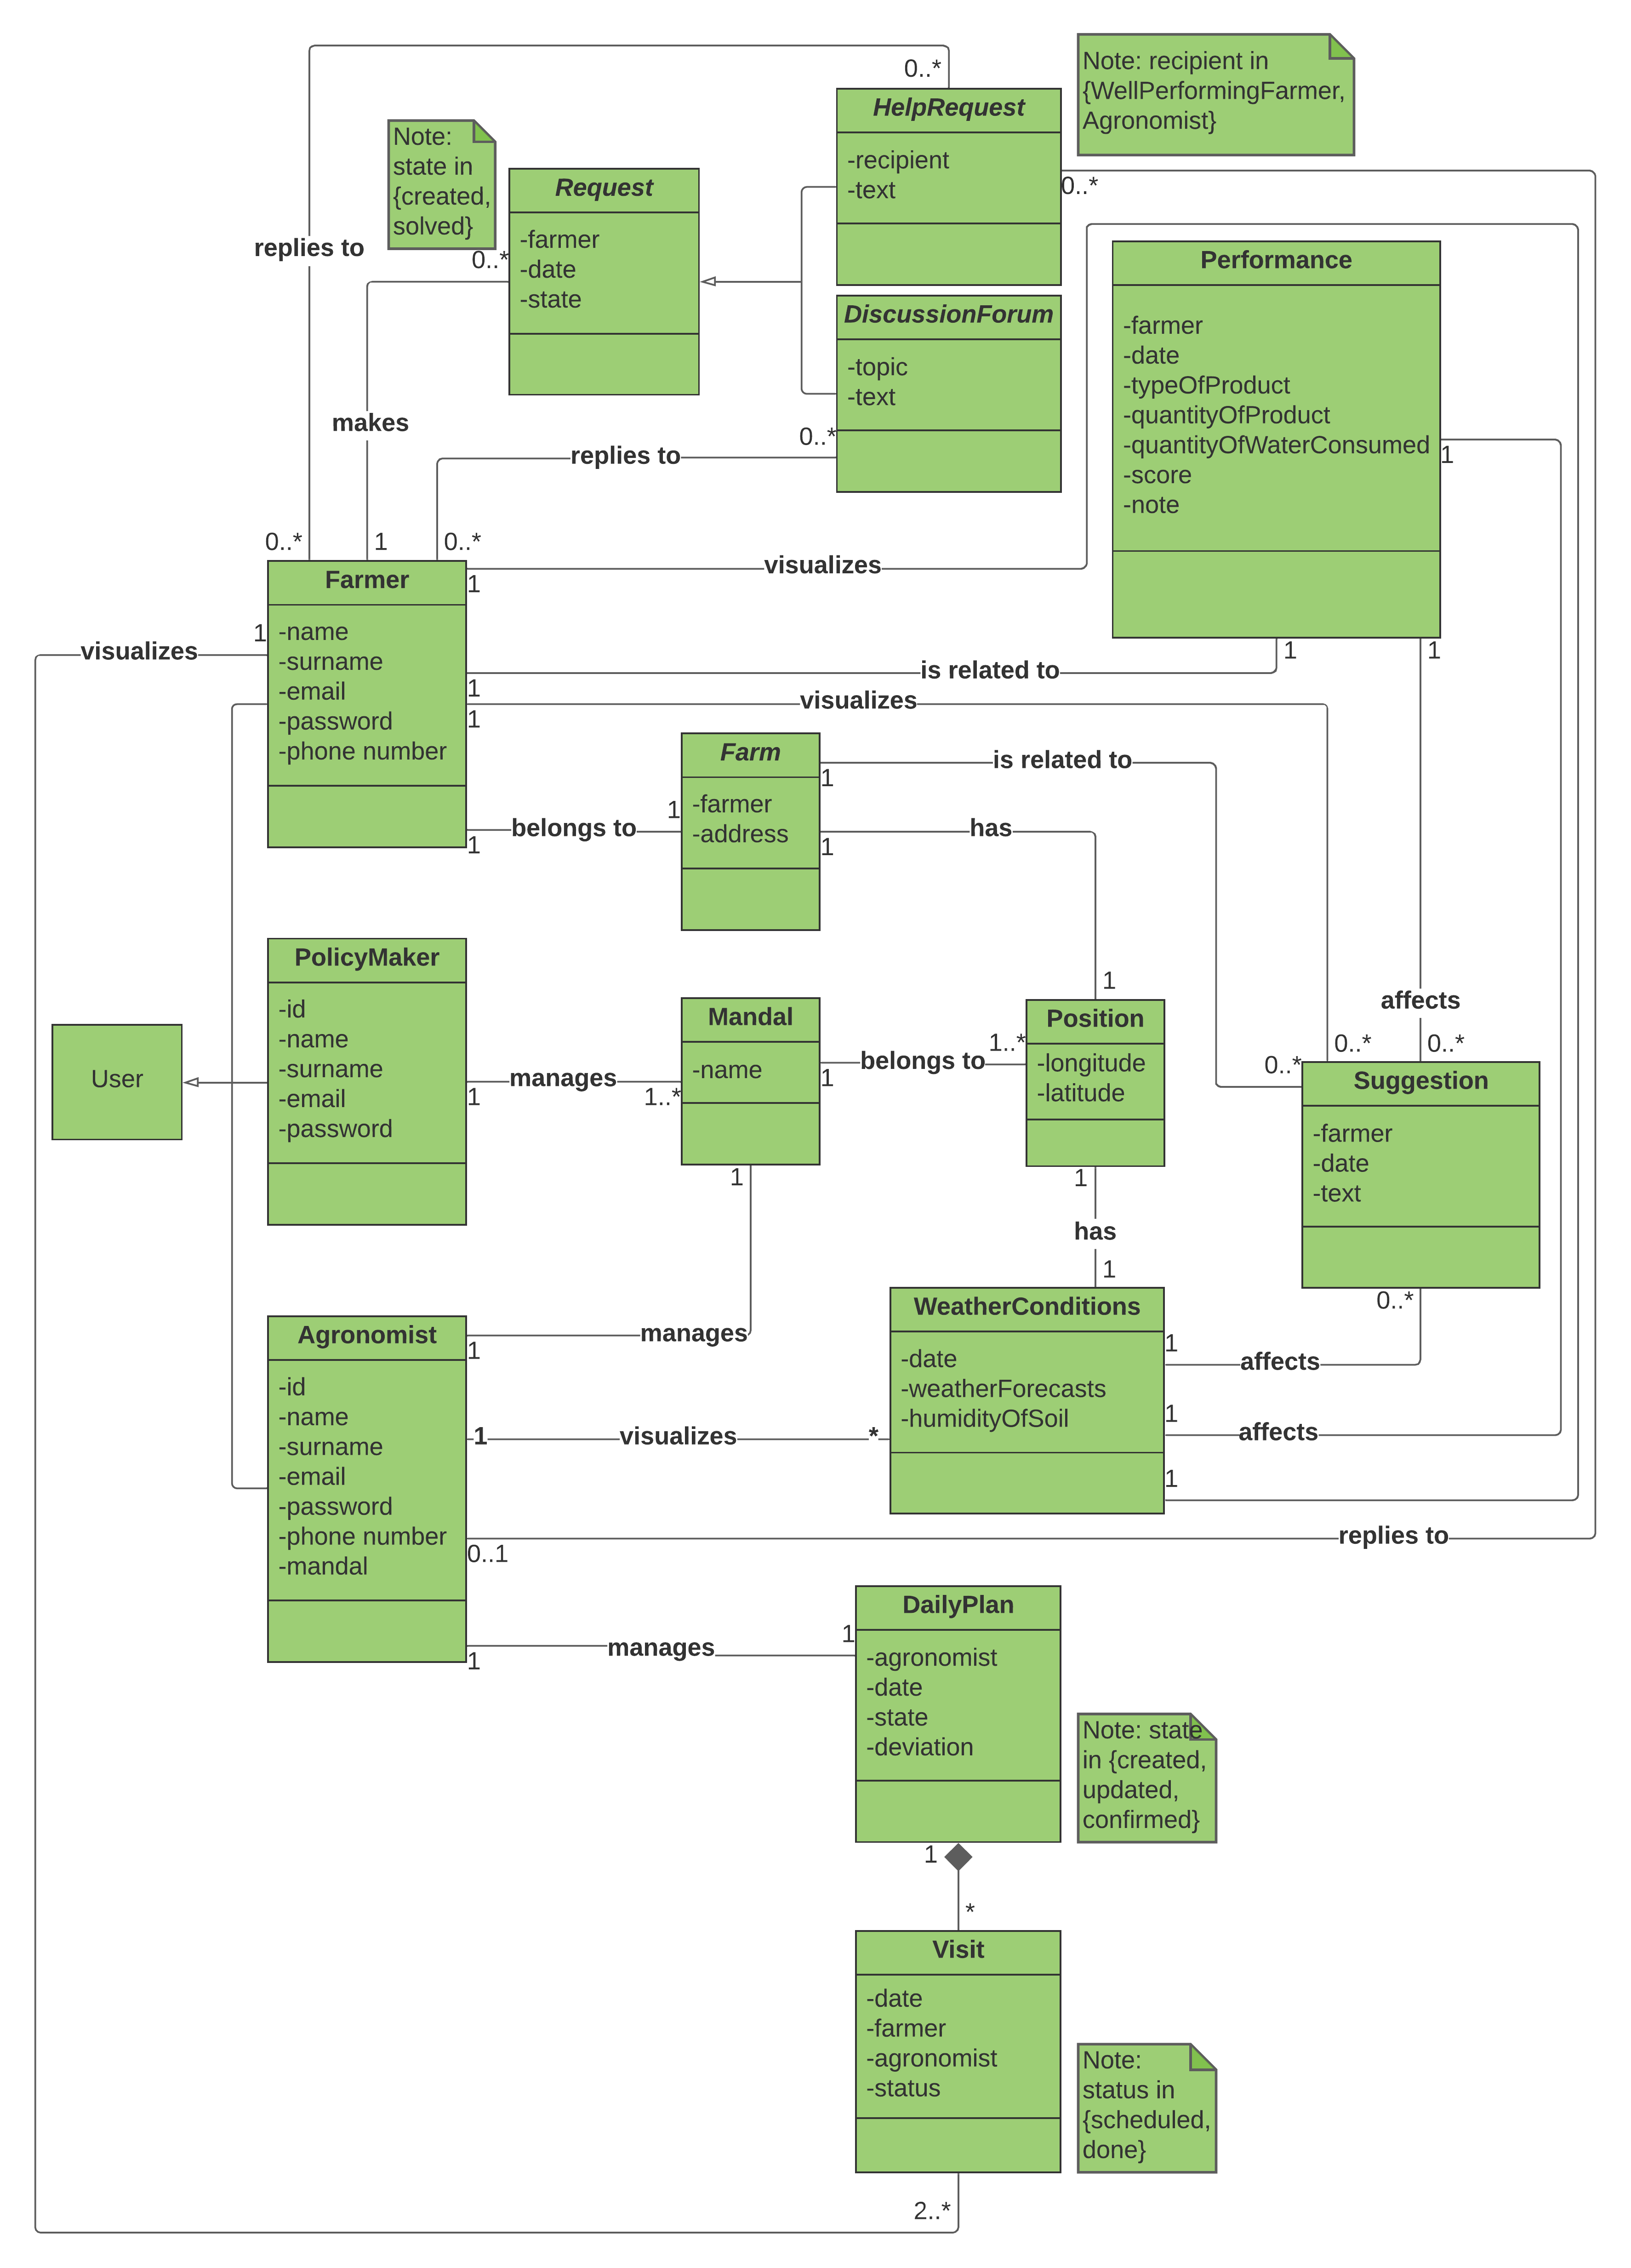
\includegraphics[width=125.5mm,scale=0.9]{./Images/Class Diagram DREAM.png}
  \caption{Class Diagram}
\end{figure}





\newpage



\subsection{State Charts}

\subsubsection{Daily Plan State Diagram}
This state diagram shows the three states of a Daily Plan.\\
The Daily Plan is \textit{Created} by the system and then \textit{Updated} or carried out and \textit{Confirmed} by the agronomist, depending on whether he needs to change the plan or not.
\begin{figure}[h!]
  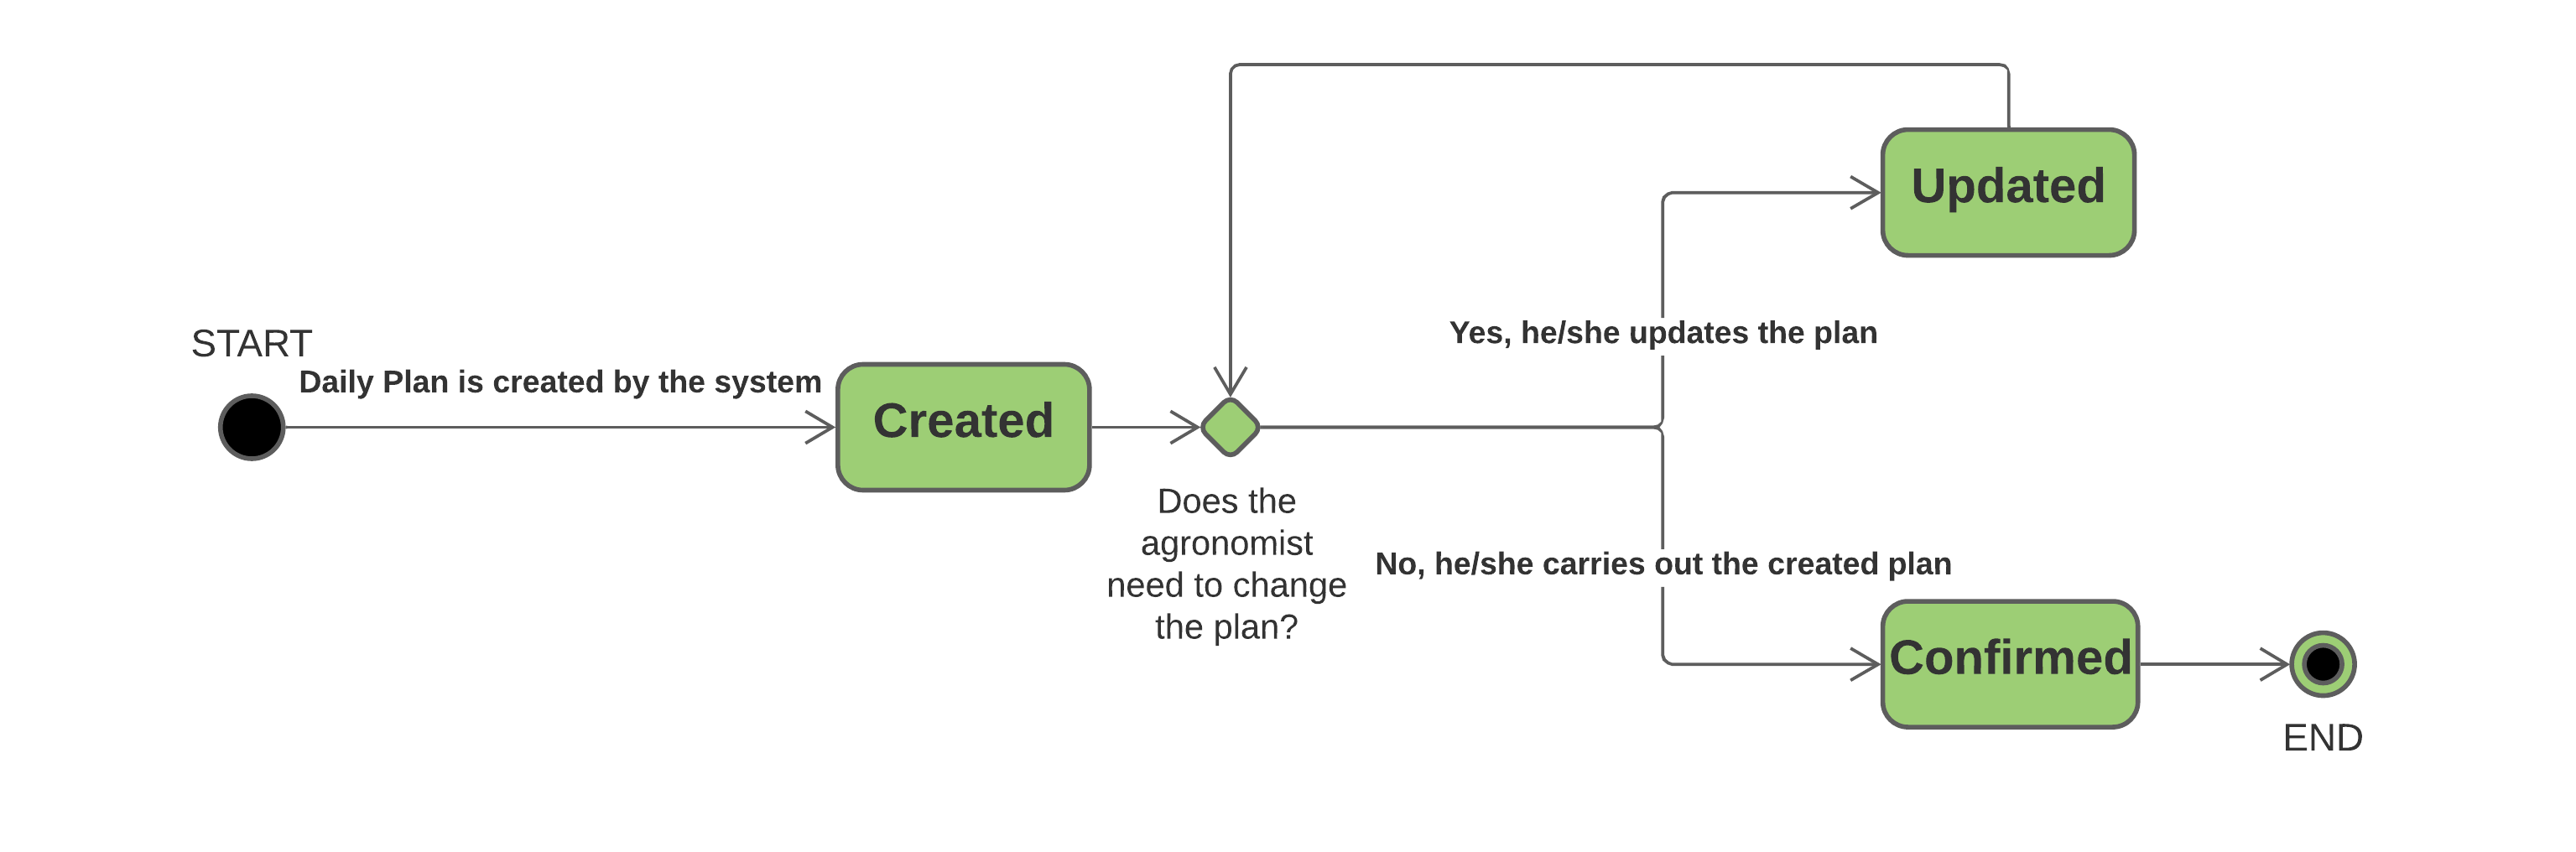
\includegraphics[width=\textwidth,height=\textheight,keepaspectratio]{./Images/State Chart DailyPlan.png}
  \caption{Daily Plan State Diagram}
\end{figure}

\subsubsection{Help Request State Diagram}
This state diagram shows the two states of a Help Request.\\
The Help Request is \textit{Created} and then \textit{Solved} by the farmer, depending on whether he is satisfied with the reply received or not.
\begin{figure}[h!]
  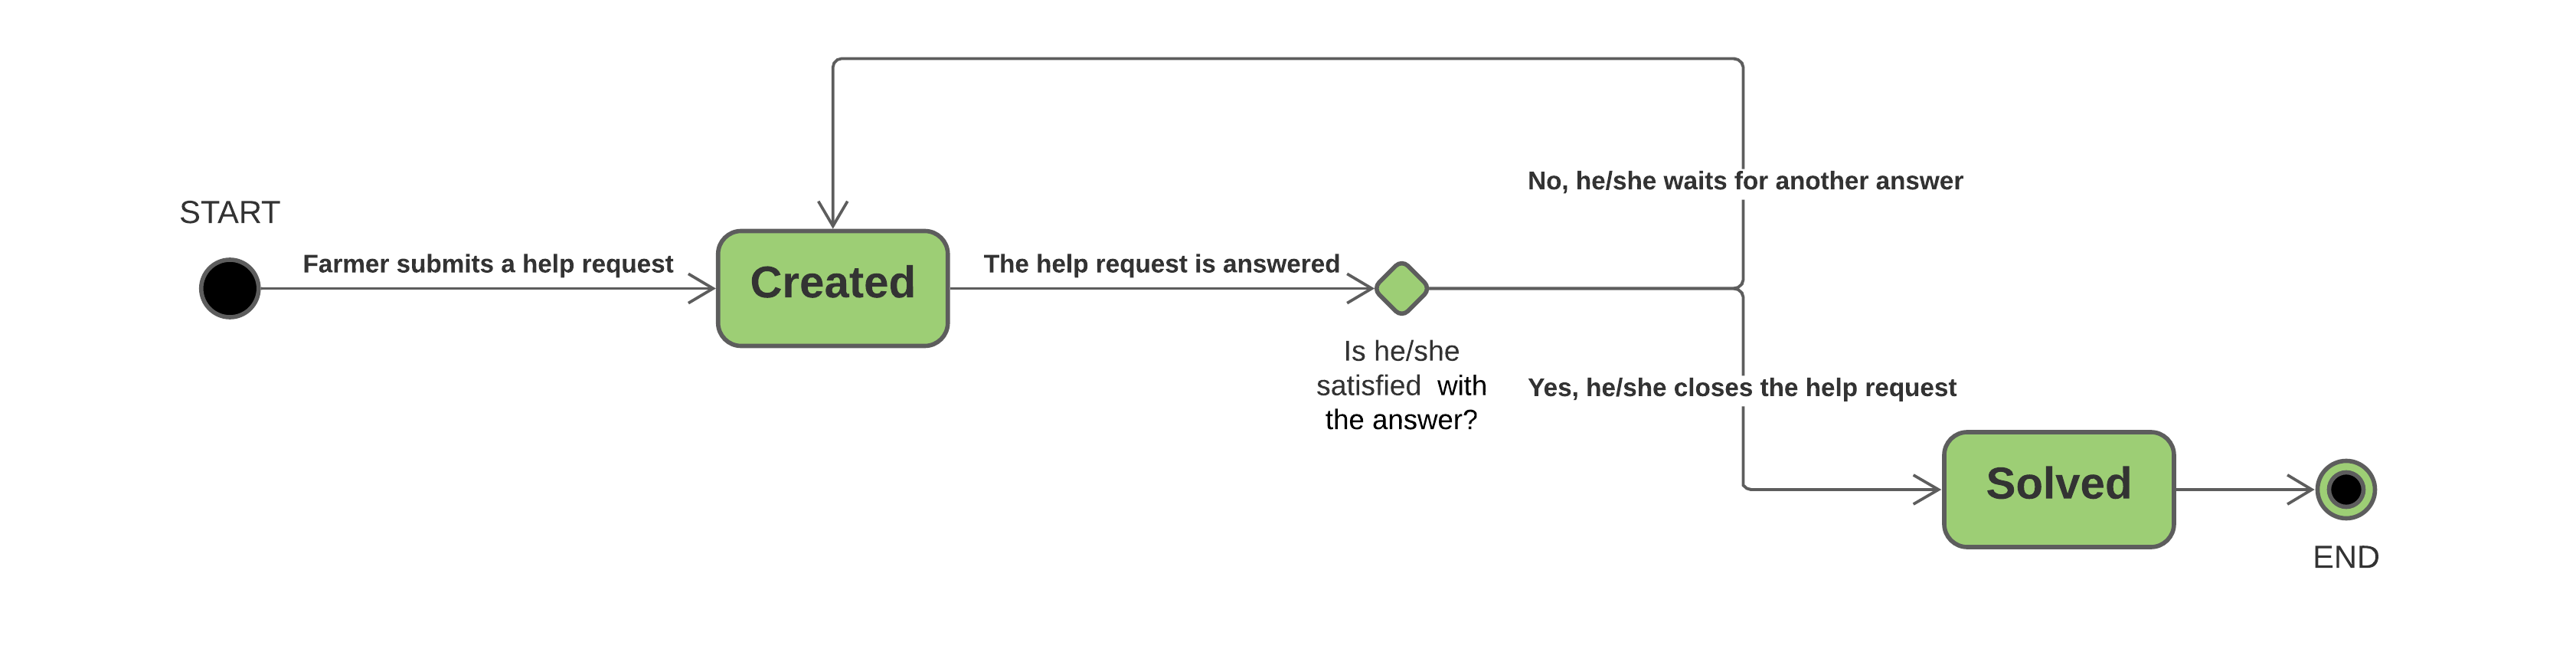
\includegraphics[width=\textwidth,height=\textheight,keepaspectratio]{./Images/State Chart HelpRequest.png}
  \caption{Help Request State Diagram}
\end{figure}

\subsubsection{Discussion Forum State Diagram}
This state diagram shows the two states of a Discussion Forum.\\
The Discussion Forum is \textit{Created} and then \textit{Solved} by the farmer, depending on whether he is satisfied with the replies received or not.
\begin{figure}[h!]
  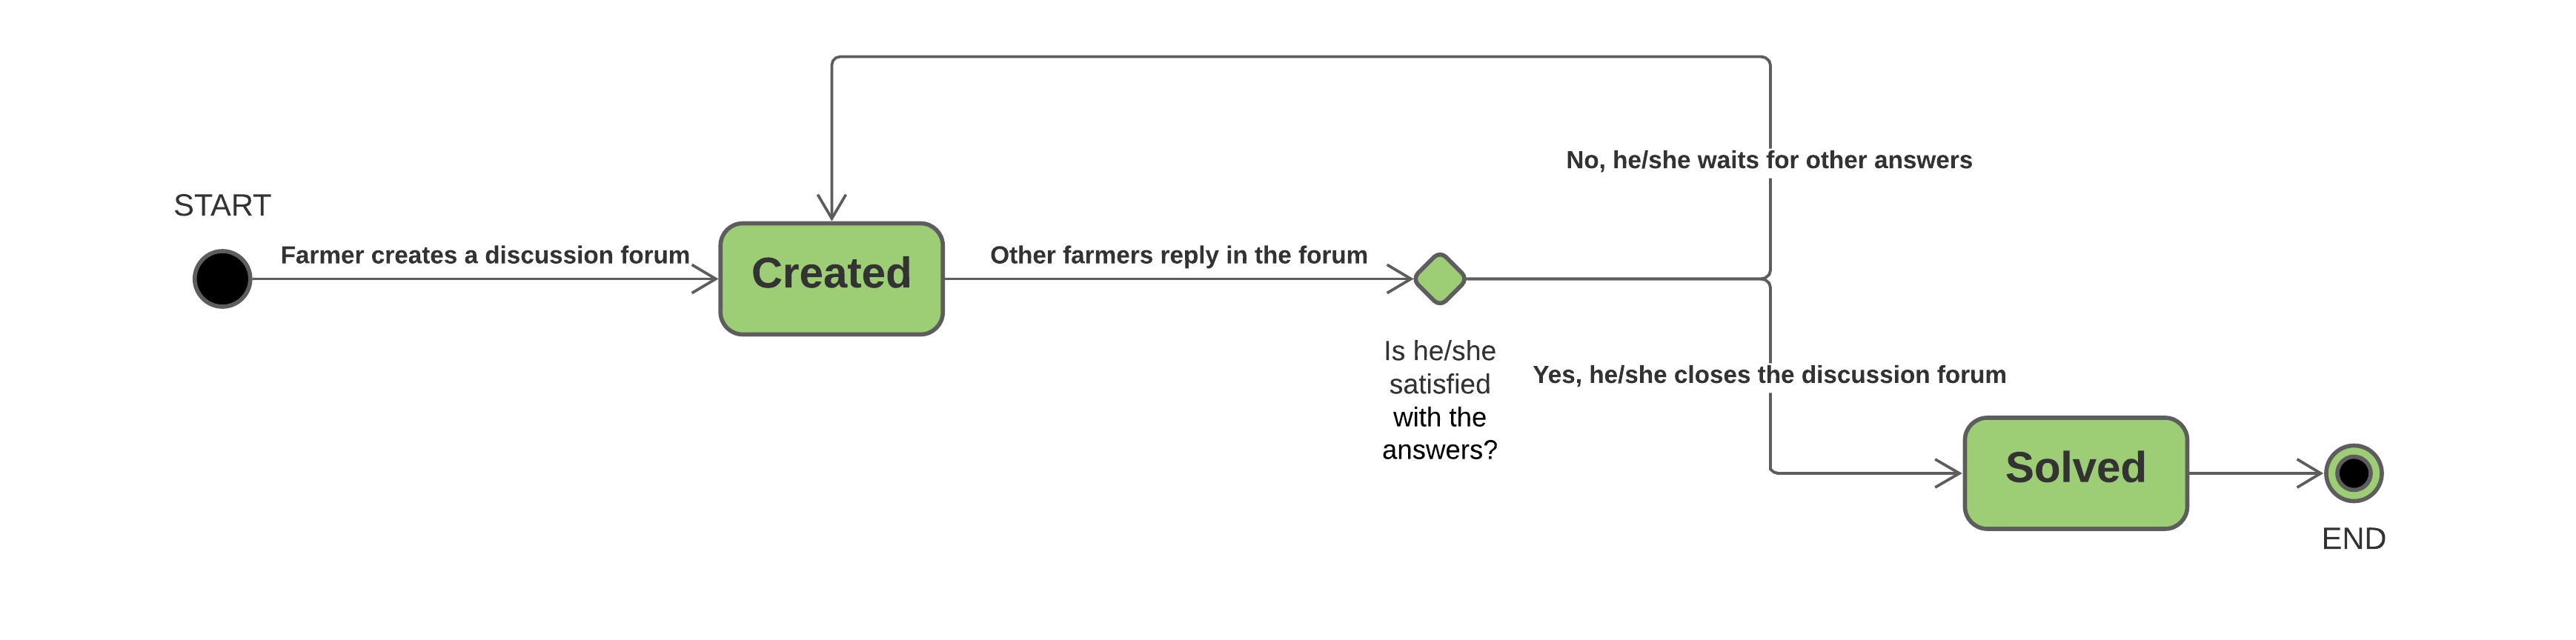
\includegraphics[width=\textwidth,height=\textheight,keepaspectratio]{./Images/State Chart DiscussionForum.png}
  \caption{Discussion Forum State Diagram}
\end{figure}

\subsubsection{Visit State Diagram}
This state diagram shows the two states of a Visit.\\
The Visit is \textit{Scheduled} and then \textit{Done} after the agronomist carries out the visit and confirms the corresponding Daily Plan.
\begin{figure}[h!]
  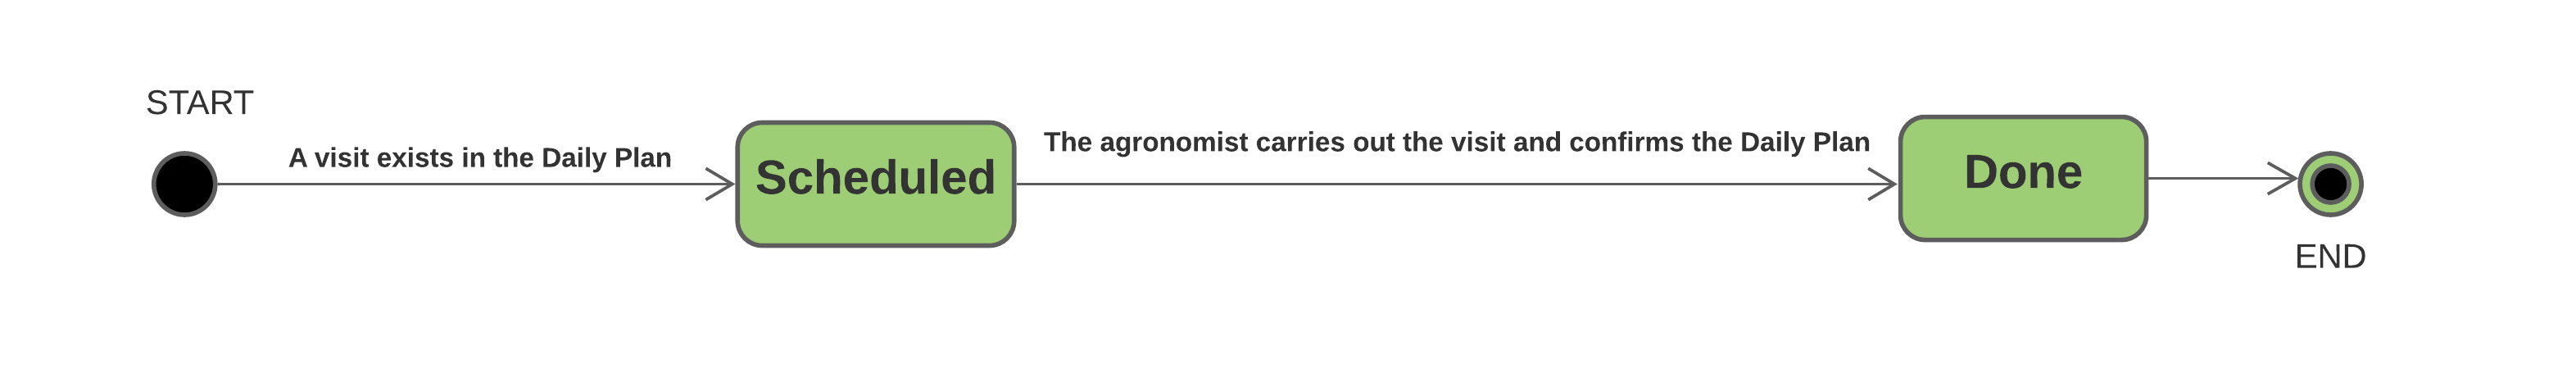
\includegraphics[width=\textwidth,height=\textheight,keepaspectratio]{./Images/State Chart Visit.png}
  \caption{Visit State Diagram}
\end{figure}
